\chapter{Introduction}

This report documents the work done in relation with project in DTU
course 02285 on ``Artificial Intelligence''.  This particular project
explores the use of AI (Artificial Intelligence) in the context of the
Sokoban game.

\section{Background and Rules}
\label{sec:rules}

Sokoban (means Warehouskeeper) was created in 1980 by Japanese
software company. The object of the game is to place boxes on goal
squares (their storage location).  Each level consists of a number of
goal squares and a corresponding number of boxes sorrounded by a
wall. This is called the floor plan (or board). To achieve the
objective, the user is represented with as a player able to move in
the directions: up, down, left and right. Boxes can not be pulled,
only pushed. \citep{cgw:sokoban}


Player and boxes can stand on goal squares. If a wall occupies a space
nothing else can be there and the wall cannot be moved from that
space.  The floor plan should be completely enclosed by a continuous
wall.

The game itself is rich in complexity and difficulty can vary from
very easy to incredibly complex, for both human players and automatic
solvers. This of course depends on the initial floor plan.

The high game complexity stems from, among other things:
\begin{itemize}
\item The game is PSPACE Complete. \cite{culberson97sokobanpspace}
\item Some game states cannot be reversed (deadlocks, pushing boxes
  against walls, etc.)
\item Up to four moves at each state. (Grows as $n^4$.)
\end{itemize}


Figure \ref{fig:soko-org-screen} shows the floor plan of the first
level original game.

\begin{figure}
  \centering
  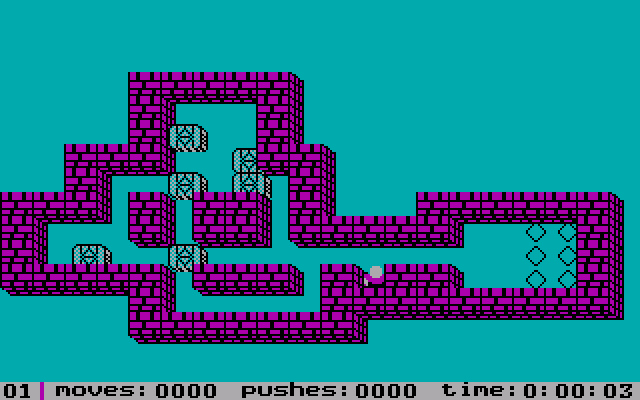
\includegraphics[width=0.7\textwidth]{sokoban-screenshot}
  \caption{Screenshot of the original Sokoban game. From Wikipedia:
    \url{http://en.wikipedia.org/wiki/Sokoban}.}
  \label{fig:soko-org-screen}
\end{figure}

\section{Problem Formulation}

The assignment leaves us rather free to choose our focus, but there are
some minimum requirements we must meet. In this list of tasks we chose
some of them to focus on and others to address more lightly.

\section{Primary Focus of the Project}
We chose to put our primary focus in the project and the report on
implementating a solver for arbitrary Sokoban floor plans.

This means that large parts of this report will deal with the design
and implemenation of such a solver and especially the heuristics used 
by the solver will be put in focus.

This also implies that we to a lesser degree address the more academic
studies of complexity in the game.

We will implement at least 3 different techniques for solving the
Sokoban challenges:
\begin{itemize}
\item Simple breadth first progression planner. %done
\item An \astar progression planner, only using a general heuristic. %done
\item The same as above, replacing the general heuristic with one we
  design ourselves with the Sokoban game in mind.
\end{itemize}



\section{Scope Limitation}
\label{sec:scope}
\subsection{Implementing Sokoban Variants}
We will not try to implement the multi-agent variant of Sokoban in our
solver implementation, since we feel that solving solving the original
problem is already a rather large challenge. As an example it took
among others a full-time Ph.D. student, full-time summer student and a
part-time proffessor two years to implement a Sokoban solver that
could solve 52 of the standard 90 puzzles that come with the
game. \citep{Junghanns99domain-dependentsingle-agent}

Furthermore we will not vary the rules in the implementation, e.g. by
adding colors to boxes and goals, adding trap doors or allowing
several boxes to pushed simultaneously. Adding these variants would
require us to change our underlying model.

\section{Structure of Report}


First we develop a STRIPS formulation of Sokoban (Chapter
\ref{cha:strips}). This description will be used in Chapter
\ref{cha:design} to construct an executable model of the game along
with a breadth-first solver. In Chapter \ref{cha:heuristics} we define
the heuristics needed to guide the search. We then continue to analyse
our findings in Chapter \ref{cha:analysis}. Chapter
\ref{cha:discussion} is where we discuss the improvements and more the
solver could benefit from. Finally in Chapter \ref{cha:conclusion} we
conclude this report.


